\documentclass[a4paper,10pt]{scrartcl}
\usepackage[utf8]{inputenc}
\usepackage[ngerman]{babel}
\usepackage[T1]{fontenc}
 \usepackage{parskip}
\usepackage{graphicx}
\usepackage{booktabs}
\usepackage{tabularx}
\usepackage{comment}
\usepackage{pdflscape}
\usepackage{url}
\usepackage{listings}
\usepackage{color}
\usepackage{multicol}

\usepackage[usenames,dvipsnames,svgnames]{xcolor}


\usepackage{geometry}
\geometry{a4paper, top=25mm, left=40mm, right=25mm, bottom=30mm,
headsep=10mm, footskip=12mm}

\definecolor{mygreen}{rgb}{0,0.6,0}
\definecolor{mygray}{rgb}{0.5,0.5,0.5}
\definecolor{mymauve}{rgb}{0.58,0,0.82}

\lstdefinestyle{customc}{
  belowcaptionskip=1\baselineskip,
  breaklines=true,
  frame=L,
  xleftmargin=\parindent,
  language=C,
  showstringspaces=false,
  basicstyle=\footnotesize\ttfamily,
  keywordstyle=\bfseries\color{green!40!black},
  commentstyle=\itshape\color{purple!40!black},
  identifierstyle=\color{blue},
  stringstyle=\color{orange},
}

\lstdefinestyle{customasm}{
  belowcaptionskip=1\baselineskip,
  frame=L,
  xleftmargin=\parindent,
  language=[x86masm]Assembler,
  basicstyle=\footnotesize\ttfamily,
  commentstyle=\itshape\color{purple!40!black},
}

\lstset{escapechar=@,style=customc}

\title{Proseminar Praktische Informatik, BSP-Programmiermodell}
\author{Danny Hofmann}


\begin{document}
\tableofcontents
\newpage

\section{Einleitung}
%TooooooooooooooooooooooooooooOODO ABSÄTZE

Paralleles Rechnen stellt Informatiker, Mathematiker und Elektrotechniker vor viele Herausforderungen. Zum einen muss die entsprechende Computer-Hardware dafür ausgelegt sein, effizient und problemlos parallele Probleme zu lösen. Zum anderen muss eine entsprechende Programmiergrundlage existieren damit eine gegebene Hardware-Plattform auch auf einer hohen, abstrakten Programmierebene angesprochen werden kann[1].\\
Der rasante Fortschritt der Computer-Hardware ermöglicht es, dass es heutzutage recht einfach und günstig ist, ein paralleles System anzuschaffen. Mit dem Einsatz von Multicore-Prozessoren in Endbenutzer Hardware sind auch die ersten parallelen Ansätze in der Mitte der Gesellschaft angekommen. Mit dem Voranschreiten der Prozessortechnik und der damit einhergehenden hohen Taktung, ist es möglich sehr viele Befehle pro Sekunde auszuführen. Demzufolge muss ein Konzept erfunden werden, welches möglichst viele Befehle für den Prozessor erzeugt aber nur wenig Programmier-/Schreibarbeit für den Programmentwickler bedeutet.\\
Im Sinne dieser Seminararbeit, wird im folgenden ein Programmiermodell zur Behandlung von Parallelen Problemen behandelt. Das Bulk Synchronous Parallel (BSP) Modell, dies steht für Massensynchrone Parallelrechner welches den Ansatz hat, dass ein Vielzahl von Prozessoren ihren eigenen Speicher haben(MIMD-Multiple Instruction Multiple Data)[2]. Im folgenden werden einige Grundprinzipien des BSP erläutert und anhand eines simplen Programmierbeispiels anschaulich am Code erklärt.  

\section{Programmiermodell}
Ein Programmiermodell ist eine Notwendige Abstraktion der Hardware. Es schlägt die Brücke zwischen der eigentlichen Programmiersprache und der zugrundeliegenden ausführenden Hardware[6]. Es ist sinnvoll Abstraktionsebenen zu bilden, man möchte den Programmierer entlasten und die Maschine aber dafür auslasten.
\\
\\
Ein Programmiermodell sollte auch gewissen Ansprüchen genügen, wie in [1] gezeigt gibt es 4 Anforderungen an ein Programmiermodell:
\begin{itemize}
\item Übertragbar - Ein Programm sollte ohne eine komplette Umstrukturierung, oder auch ohne neu Design auf eine andere Plattform übertragbar sein.
\item Effizient - Modelle sollen die Gesamte Leistung, Möglichkeiten des Parallelensystems ausnutzen.
\item Einfachheit - Je Einfacher das Modell gehalten ist, mit seinen Befehlen und Regeln, umso einfacher ist es für einen Programmierer schnell, fehlerfreien und damit auch effizienten Code zu schreiben.
\item Berechenbare Laufzeit - Die Laufzeit eines Codeentwurfs vorauszuberechnen, ist essentiell dafür um aus vielen Möglichkeiten, ein Problem zu Implementieren, die beste herauszufinden.
\end{itemize}
Im folgenden wird das Programmiermodell BSP vorgestellt, welches jede oben genannte Eigenschaft besitzt. Ein Programm welches dem BSP-Modell zugrunde liegt, ist auf jedes BSP geeignete Verteiltesystem portierbar. Es wird die möglichkeit gegeben Rechenlast gleichmäßig über das System zu verteilen. Dem BSPlib Standard liegen nur rund 20 Befehle zu Grunde[5], demzufolge ist es recht überschaulich gehalten und erfüllt den Punkt der Einfachheit. Zuletzt besitzt der BSPlib Standard ein Rechenmodell womit die Performance eines Systems unter bestimmten Umständen bestimmt werden kann.
\newpage
 
\section{Bulk Synchronous Parallel}
\subsection{Geschichte}
\begin{minipage}{0.6\textwidth}
Das Modell BSP wurde von einem Britischen Informatiker namens Leslie Valiant, an der Harvard Universität entwickelt. Über die 1980er Jahre entwickelte er seine Vorstellung über ein Paralleles Programmiermodell was davon ausging, dass eine Kommunikation und Synchronisation in einem Parallelen Rechner nicht gleich gegeben oder sogar trivial ist[3]. Nachdem Valiant seine Arbeit 1990 veröffentlichte arbeitete er mit Bill McColl an der Verfeinerung seiner Ideen und Konzepte. 
McColl führte Mitte der 1990er Jahre ein Internationales Forscherteam an der Oxford Universität. 1997 veröffentlicht McColl seine Arbeit in einem Standard der heutzutage als Oxford BSPlib Standard bekannt ist[4]. In den folge Jahren gibt es verschiedene Umsetzung dieses Standards und auch einige Erweiterungen. Der Oxford BSPlib Standard, fand seine erste Implementierung in Fortran und wurde später in heutzutage gängigen Programmiersprachen implementiert, wie C,C++ oder Java[5].
\end{minipage}
\begin{minipage}{0.4\textwidth}

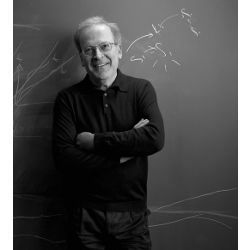
\includegraphics[scale=1.3]{LeslieValiantBW.png}
\captionof{figure}{Leslie Valiant}



\end{minipage}
\subsection{Aufbau einer BSP Maschine}
Um ein BSP-System zu Implementieren werden zunächst einige Dinge benötigt, zum einem handelt es sich um einen MIMD Ansatz, also benötigt man mehrere Prozessoren die einen dedizierten Speicher haben.[1]\\
Im BSP wird auch eine Kommunikation zwischen den Prozessoren, oft in einem Netzwerk, benötigt. Wie man dieses Netzwerk gestaltet liegt zunächst in der Hand des Systemerstellers. Um eine Datenübertragung zwischen den Prozessoren zu gewährleisten müssen die Verbindungen über einen Router laufen, der dafür sorgt das die Prozessoren sich untereinander verständigen können. Die Kommunikation ist getrennt von jeglicher Synchronisation. Die Synchronisation ist teil der Barriere welche garantiert, dass der Datenaustausch zwischen den Prozessoren abgeschlossen ist und erst dann die übertragenen Daten für den einzelnen Prozessor zugänglich werden. Demzufolge arbeiten alle Prozessoren erst weiter, wenn der Datenaustausch abgeschlossen ist. Diesen Vorgang nennt man im BSP-Modell "Barrier-Synchronisation".[1]

\subsection{BSP Algorithmen}
Wie man schon aus dem Aufbau einer BSP Maschine erkennen kann, besteht auch der Algorithmus eines BSP Programmes aus 3 Teilen. Wie in Abbildung 2 gezeigt wird zuerst die Rechenarbeit die jedem Prozessor zugeteilt wurde abgearbeitet, dann beginnen die Prozessoren untereinander Daten zu verschicken und im letzten Schritt werden diese Daten dann lokal für die einzelnen Prozessoren sichtbar. Diesen Ablauf nennt man einen \textit{Superstep}.\\
Ein BSP-Algorithmus besteht aus einem oder mehreren Supersteps. In einem Superstep werden möglichst viele Aktionen bzw. Befehle versucht unter zu bringen, damit man alle verteilten Prozessoren möglichst gut auslasten kann, daher auch "Bulk" zu deutsch "Masse oder auch großes Bündel".  	


\begin{figure}[h]
	\centering 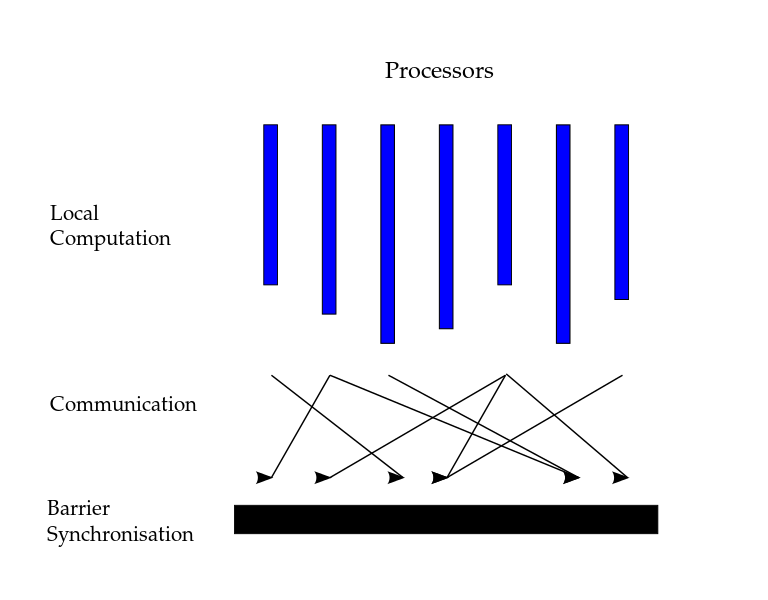
\includegraphics[scale = 0.4]{superstep.png}
	
	\caption{Ein Superstep}
\end{figure}

\newpage

\subsubsection{Kommunikation}
Die Kommunikation in einem BSP-System ist zu teilen mit der Kommunikation in einem verteilten System zu vergleichen. Dabei kann man auch verschiedene Ebenen betrachten, Senden und Empfangen einer Nachricht, oder direkter Speicher Austausch. In BSP wird werden alle Nachrichten sofort und ohne Verzögerung versendet. So eine "Massenversendung" hat den Vorteil, dass man eine Obergrenze an Zeit festlegen kann, die eine Kommunikation benötigt und damit zur Berechenbarkeit beiträgt. 

\subsubsection{Barriere}
Die Strukturierung weg von einer einheitlichen Kommunikation und Synchronisation zur Trennung eben dieser Beiden in Kommunikation und Barrierensychronisation, sieht auf den ersten Blick unnötig aufwändig und kompliziert aus. Wenn man sich aber näher mit den Nachteilen eines einheitlichen Datenaustauschs mit Datenverarbeitung beschäftigt kommt man schnell auf das allgemeine Problem des Deadlocks, oder 	einer anderen Form den Livelock. In BSP geht man diesem Problem der Prozessverklemmung komplett aus dem Weg, eben weil eine Barriere keine Ringförmigen Abhängigkeiten zwischen Daten kreieren kann[4].\\
Die Optimierung der Barriere ist in einem BSP-System essentiell da, an einer gut Implementierten Barriere die Performance des Systems steht oder fällt. Die StandardBSPlib benutzt als simplen Optimierungsschritt einen Overhead bei den Datenpaketen der den einzelnen Prozessoren sagt wie groß die Pakete sind die er empfängt. Solch ein Ansatz erhöht den benötigten Speicher und die Größe der Nachricht nur minimal, erhöht aber das Potential für Optimierungen enorm. Jeder Prozessor weiß nun wie groß die Pakete sind die er Empfangen wird. Das macht es einfacher Einstellungen bei der Programmierung der Barriere zu setzen[1].
\newpage

\subsubsection{Code Beispiel}
Im folgenden wird an einem Code Beispiel der Ablauf eines BSP Algorithmus deutlich erklärt. Verwendet wurde dabei eine Bibliothek von Albert-Jan N. Yzelman, welche er in seiner Promotion entwickelte und auch später weiter führte. Die Entwickelte Bibliothek MulticoreBSP für Java und C, ermöglicht es auf modernen Mehrkernprozessoren ein BSP System zu implementieren[7].\\
Hier wurde ein Simpler Ansatz gewählt um die Vorgehensweise zu verdeutlichen. Es wird in einem Superstep über zwei Prozessoren zunächst die Oberfläche und das Volumen einer gegebenen Kugel berechnet. Nach diesem Superstep wird eine Barrierensynchronisation durchgeführt und der erste Prozessor berechnet dann im zweiten Superstep wie viele dieser Kugeln in einen Kubikmeter Würfel passen. Folgender Code wurde auf einer vier Thread CPU ausgeführt.
\begin{lstlisting}
#define _PI 3.14159265358979323846 /*pi*/
#define circumference 10.0f
static double rad = circumference / (2 * _PI);
   
\end{lstlisting}
Zuerst werden benötigte Variablen Global in C definiert, PI und der Durchmesser der Kugel. Alle Threads können nun darauf zugreifen, vereinfacht die Anschaulichkeit des Beispiels.

\begin{lstlisting}
    double a = 0.0;
    
    bsp_begin(1);//Creates Thread 0  
    //Registers memory location for communication  
    bsp_push_reg(&a, sizeof(double));   
    bsp_init(&spmd2_entry, 0, NULL);//prepares Entrypoint for spmd2    
\end{lstlisting}
Variable a wird für BSP als Globale Variable Register, worauf dann auch eine Barrieren Synchronisation zugreift. Es wird dann Thread 0  erstellt dieser ermöglicht nun, den ersten Superstep einzuleiten.

\begin{lstlisting}
void spmd2_entry(void)
{    
    bsp_begin(2); //Generate 2 Threads
    double local = 0.0f;//local memory
    if(bsp_pid() == 1)//Thread 1 Calculates the Sphere volume
    {       
        local = (4/3) * _PI * (rad*rad*rad);
        bsp_push_reg(&local, sizeof (double) ); // Registers memory location for communication
    }    
    else //Calculates Area
    {   local = 4 * _PI * (rad * rad);
        bsp_push_reg(&local, sizeof (double) );
    }    
    bsp_sync();//signals the end of a Superstep and starts global communication
    bsp_end();//ends the called thread by bsp_begin()
} 

\end{lstlisting}
Nachdem im Thread 0 der Superstep eingeleitet wird, beginnt zuerst die lokale Berechnung der einzelnen Threads/CPUs hier rechnen zwei Threads parallel. Beide Threads haben einen lokalen Speicher. Thread 1 berechnet das Volumen der Kugel und Thread 2 die Fläche. Mit bsp\_sync wird dann die Barrierensynchronisation eingeleitet. Beide Threads übergeben nun ihre lokalen Daten an die Barriere. Hier wurde dies durch ein n-Thread großes Array gelöst, Thread 0 schreibt in Element 0, Thread 1 in Element 1 und so weiter.

\newpage

\begin{lstlisting}
void spmd2_p0(double * const a)
{
 /*write Data of Threads in array*/
    for(unsigned int s = 0; s < bsp_nprocs(); ++s)
    {
        bsp_direct_get(s,array,0,array + s, sizeof(double));
        
        printf("Thread %d has result: %lf\n", s, array[s]);
        
       *(a+s-1) = array [s]; 
   }
    
    free(array);
}
\end{lstlisting}
In der Anfangs definierten Globalen Variable a wird nun der Feldeintrag geschrieben der für die weitere Berechnung erforderlich ist.

\begin{lstlisting}
if(bsp_pid() == 0){
    
	    printf("\nThread 0 calculates how many spheres will fit in an cubic 1 m cube...\n");                 
        bsp_direct_get(0, &a, 0, &volumeSphere, sizeof(double));}//get data from thread 1     
    
        /*cubic 1m = 1 000 000 cubic cm under the assumption the spheres will fill approx. 60% of the given space there is a volume of 600 000 cubic cm to fill*/
        /*Thread 0 calculates how many Spheres will fit in a cubic 1m square*/
        int volumeFit = 600000 / volumeSphere;
        printf("cubic 1m will be filled approx. by %d spheres with %.4f cm circumference.\n", volumeFit, circumference);
    
    bsp_end();
\end{lstlisting}
Zurück in Thread 0 wird nun die Globale Variable a mit den Errechneten Werten aus dem vorhergehenden Superstep in einem neuen, dem	 zweiten,  verwendet um zu berechnen wie viele dieser Kugeln mit dem berechneten Volumen in einen Kubikmeter Würfel passen.Als letzten Schritt wird errechnete Anzahl noch auf dem Bildschirm ausgegeben und der zweite Superstep kommt zu einem Ende.	
\newpage

\subsection{Optimierung}
Ein Programmierer ist immer dazu angehalten die Laufzeit seines Systems, und eben auch seines Codes, so klein wie möglich zu halten. Unter der BSPlib gibt es auch einige Ansätze der Optimierung, so wird das Programm eher kaum in den Fokus einer Optimierung gesetzt. Der Großteil der Optimierung findet in der abstrakten BSP Maschine statt und da vor allem in der Kommunikation zwischen den Prozessoren. Im folgenden werden einige implementierte Verbesserungen der BSPlib vorgestellt.

\subsubsection{Message Packing}
Um die Netzwerklast zu minimieren packt man bei Message Packing mehrere Pakete, die an zwischen zwei Netzwerkteilnehmern verschickt werden, zu einem zusammen. Das Kostenmodell von BSP fordert, dass eine Nachricht von zB. 500-byte genauso viel Speicher und Zeit kosten soll, wie 500 1-byte große Nachrichten. Um diesen Grundsatz zu erfüllen setzt man in der BSPlib Message Packing ein, demzufolge wird der Overhead einmal pro Prozessorpaar beansprucht und nicht bei jeder Nachricht erstellt.

\subsubsection{Destination Scheduling}
Wie vorher erklärt treten die Prozessoren alle gleichzeitig in die Kommunikation über, also wenn ein Prozessor anfängt Daten zu versenden werden die anderen eben so ihre Daten losschicken. Angenommen alle Prozessoren wollen als ersten Kommunikationsschritt etwas an Prozessor 1 schicken, so ist dieser Prozessor sichtlich schnell überlastet und das Netzwerk fällt in einen Busy-Wait. So ein Vorgehen ist in anderen SPMD Programmiermodellen, oft der Fall und führt daher auch zu Problemen. Die BSPlib geht an solch ein Bomberdamen von Anfragen an einen Prozessor anders um. Zum einen ist die Reihenfolge wie Nachrichten versandt werden nicht festgelegt, sie wird zufällig bestimmt[1]. Dadurch ist die Wahrscheinlichkeit einer auftretenden Massen Kollision nahezu gebannt und wirkt sich sehr positiv auf die Performance aus.
\subsubsection{Pacing}
Ein Netzwerk besteht aus vielen Komponenten, oft behindern sich einige gegenseitig und Formen einen Engpass, oder auch Bottleneck. Ein Bottleneck kann bis zu einer bestimmten Höhe an Transaktionen vollkommen ohne Auswirkungen für ein System sein, nur mit ansteigender Transaktionsrate in dem Netzwerk, steigt auch die Gefahr das ein Bottleneck Einfluss auf die Performance nimmt, oder sogar zu einem Totalausfall führen kann. Um so etwas vorzubeugen benutzt man Pacing. Pacing ist eine Drosselung des Systems, kurz unterhalb der maximal möglichen Übertragungsrate in diesem System. So ist gewährleistet, dass das System nicht in eine Situation kommt auszufallen, es ist im schlimmsten Fall langsam.

\section{Netzwerke in BSP}
\begin{itemize}
\item Erklärung von TCP/IP mit Bezug auf BSP
\begin{itemize}
\item Packing
\item Destination Schedule
\item Bestätigungen(Acknowladgment)
\item Fehler Verträglichkeit(Error recovery)
\end{itemize}
\item Was wird durch BSP wie optimiert.

\end{itemize}
\section{BSP in der Softwareentwicklung}
\begin{itemize}
\item Datamining(Bagging)
\item Neurale Netzwerke und Logic Programming
\item Eigene Praktische Aufgabe
\end{itemize}
\section{Fazit}
\begin{itemize}
 \item Vorteile
 \item Nachteile
 \item Resümee Nutzen
\end{itemize}
\section{Referenzen}
\begin{itemize}
\item [1] R.Correa et al (eds), Models for Parallel and Dirstibuted Computation. Theory, Algorithmic Techniques and Applications S.: 85-115
\item [2] \url{https://de.wikipedia.org/wiki/Massively_Parallel_Processing} (Abruf 01.01.2017)
\item [3] Leslie G. Valiant, A bridging model for parallel computation, Communications of the ACM, Volume 33 Issue 8, Aug. 1990 
\item [4] \url{http://www.cse.unt.edu/~tarau/teaching/parpro/papers/Bulk%20synchronous%20parallel.pdf} (Abruf 01.01.2017)
\item [5] \url{http://www.bsp-worldwide.org/implmnts/oxtool/}
\item [6] \url{https://www.math.tu-cottbus.de/~kd/parallel/vorl/vorl/node18.html}
\item [7] \url{www.multicorebsp.com}
\end{itemize}
\section{Abbildungen}
\begin{itemize}
\item Abbildung 1 \url{http://cacm.acm.org/magazines/2011/6/108643-beauty-and-elegance/fulltext}
\item Abbildung 2 \url{https://upload.wikimedia.org/wikipedia/en/thumb/e/ee/Bsp.wiki.fig1.svg/768px-Bsp.wiki.fig1.svg.png}
       
\end{itemize}





\end{document}